\documentclass[oneside,openany]{amsdtx}
\usepackage[margin=.75in]{geometry}
\usepackage{graphicx}
\usepackage{float}
\usepackage{amsmath,amssymb}
\usepackage{url}
\usepackage[dvipsnames]{xcolor}
\usepackage{multicol}
\usepackage{fancyvrb}
\usepackage[allcolors=black]{hyperref}
\usepackage{tikz}
\usepackage{booktabs}
\usepackage{bm}
\usepackage{array}
\usepackage{enumitem}
\usepackage[T1]{fontenc}
\usepackage[utf8]{inputenc}
\usepackage[english]{babel}
\usepackage{listingsutf8}
\usepackage{textcomp}
\usepackage{lmodern}
\usepackage{siunitx}
\usetikzlibrary{arrows.meta,calc,fit,positioning,shapes.geometric}

\definecolor{b}{HTML}{3C78D8}
\definecolor{B}{HTML}{08357E}
\definecolor{g}{HTML}{38761D}
\definecolor{r}{HTML}{7A0101}
\definecolor{o}{HTML}{FF7F0E}
\definecolor{p}{HTML}{A64D79}
\definecolor{codegreen}{HTML}{38761D}
\definecolor{codeblue}{HTML}{000076}
\definecolor{codepurple}{HTML}{7A0101}
\definecolor{phenolicA}{HTML}{A65A2E}
\definecolor{phenolicB}{HTML}{C98A5A}
\definecolor{epoxy}{HTML}{E9C46A}
\definecolor{aluminum}{HTML}{A8B0B8}
\definecolor{gas}{HTML}{E76F51}

\lstdefinestyle{mystyle}{
  backgroundcolor=\color{white},
  commentstyle=\color{codegreen},
  keywordstyle=\color{codepurple},
  numberstyle=\ttfamily\scriptsize\color{codeblue},
  stringstyle=\color{b},
  basicstyle=\ttfamily\scriptsize,
  breakatwhitespace=false,
  breaklines=true,
  captionpos=b,
  keepspaces=true,
  numbers=left,
  numbersep=5pt,
  showspaces=false,
  showstringspaces=false,
  showtabs=false,
  tabsize=4,
  texcl=false
}
\lstset{style=mystyle,inputencoding=utf8,extendedchars=true}

\newcolumntype{L}[1]{>{\raggedright\arraybackslash}p{#1}}
\newcolumntype{M}[1]{>{\centering\arraybackslash}m{#1}}
\protected\def\code#1{\texttt{\detokenize{#1}}}
\pdfstringdefDisableCommands{\def\code#1{#1}}
\providecommand{\codepath}[1]{\path{#1}}
\newcommand{\dd}{\mathop{}\!\mathrm{d}}
\newcommand{\pd}{\partial}
\newcommand{\vect}[1]{\bm{#1}}
\newcommand{\placeholder}[1]{%
  \begin{center}
  \fbox{\begin{minipage}[c][45mm][c]{0.90\textwidth}
    \centering\color{gray}\large #1
  \end{minipage}}
  \end{center}}

\sisetup{locale=US,per-mode=symbol,range-phrase=--,range-units=single}
\setcounter{secnumdepth}{3}
\setcounter{tocdepth}{3}

\title{~\\[-2em]\sc Thermochemical Modeling of a Phenolic Liner\\
in a Solid Rocket Motor Using ANSYS Mechanical}
\author{\sc MIT Rocket Team --- M. Nichitiu --- Solid Propulsion Simulations}
\date{\sc July 15, 2026}

\begin{document}
\selectlanguage{english}
\maketitle
\begin{multicols}{2}
	{\color[HTML]{FFFFFF} .}~~~~~~~~~~~~~~~~~
\includegraphics[scale=0.1]{logos/rtlogo.pdf}\\[1em]


~\vspace{3.3em}~\\[-4.6em]{\color[HTML]{FFFFFF} .}~~~~~
\includegraphics[scale=0.2]{logos/ansys}
\end{multicols}
~\\[-1em]
\setcounter{tocdepth}{2}
\tableofcontents\vfill 
\begin{center}
\begin{minipage}{1\textwidth}
\small
\textbf{Purpose of this document.} \it This report first describes the transient
thermal model currently being run, limited to volumetric pyrolysis of the inner
phenolic layer \code{phe0}. It then proposes an extension, still entirely within
ANSYS Mechanical, to represent outgassing and discrete recession through element
removal. Fluent and propellant combustion are outside the scope of this study.
Values marked \emph{provisional} must be replaced or validated using measurements
of the material actually manufactured before any design or safety decision is
made.
\end{minipage}
\end{center}
\vfill
% ============================================================================
\section{Context: Solid Rocket Motor and Casing Layup}

\subsection{Physical Scope}

The system under study is a solid-propellant rocket motor whose casing is modeled
as four contacting coaxial tubes: an inner phenolic layer, a thin epoxy layer, a
second phenolic layer, and an aluminum shell. The geometry file contains the
bodies \code{Phenolic0}, \code{Epoxy}, \code{Phenolic1}, and \code{Alu}, which
correspond respectively to the Mechanical named selections \code{phe0},
\code{epo}, \code{phe1}, and \code{alu}. Mechanical nevertheless meshes only
an axially truncated portion of this baseline model: the radial layup is
preserved, but the reduced height simplifies the mesh and keeps the solution
time reasonable. The dimensions below describe the complete motor, so extensive
results must be scaled before extrapolation to the full motor.

The propellant is not included in the geometry. Its effect is represented by a
prescribed gas temperature and convection coefficient on the inner surface of
\code{phe0}. It should also be noted that ammonium perchlorate (AP) is the
\emph{oxidizer} in a composite propellant, not a fuel by itself. The composition
of the fuel binder, any aluminum fraction, chamber pressure, and combustion
history are not documented in the present model. Consequently, a wall heat flux
cannot be derived from first principles: the current hot-side boundary condition
remains an input that must be calibrated against a motor firing or supplied by a
separate internal-flow model.

\subsection{Dimensions Extracted from the 3D Model}

The AP214 STEP file uses meters. Its cylindrical surfaces define the interface
radii listed in Table~\ref{tab:geometry}. The model is a straight cylinder of
length \(L=\SI{1.8288}{m}\), exactly \SI{72}{in}; its bore diameter is
\SI{266.7}{mm} (\SI{10.5}{in}), and its outside diameter is \SI{304.8}{mm}
(\SI{12}{in}). The layers have a combined thickness of \SI{19.05}{mm}.

\begin{figure}[H]
\centering
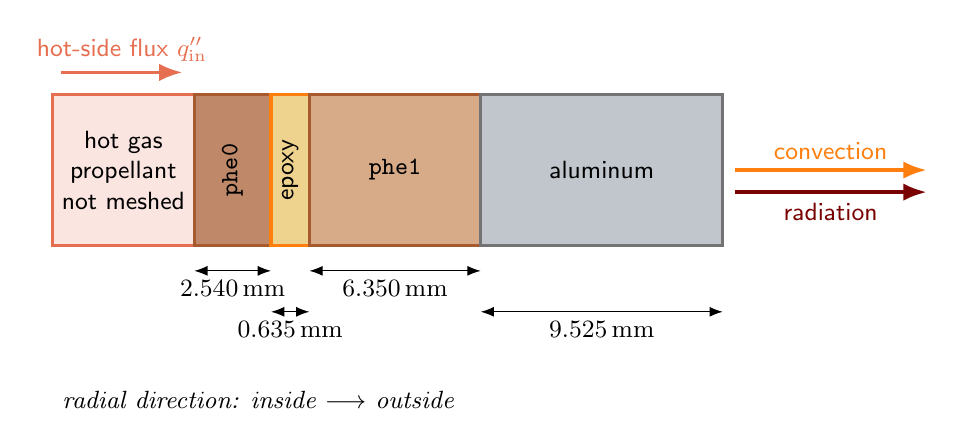
\begin{tikzpicture}[x=0.75cm,y=0.80cm,font=\sffamily\small,>=Latex]
  \draw[fill=gas!18,draw=gas,very thick] (0,0) rectangle (2.4,2.4);
  \draw[fill=phenolicA!72,draw=phenolicA,very thick] (2.4,0) rectangle (3.7,2.4);
  \draw[fill=epoxy!75,draw=o,very thick] (3.7,0) rectangle (4.35,2.4);
  \draw[fill=phenolicB!72,draw=phenolicA,very thick] (4.35,0) rectangle (7.25,2.4);
  \draw[fill=aluminum!72,draw=black!55,very thick] (7.25,0) rectangle (11.35,2.4);
  \node[align=center] at (1.2,1.2) {hot gas\\propellant\\not meshed};
  \node[rotate=90] at (3.05,1.2) {\code{phe0}};
  \node[rotate=90] at (4.025,1.2) {epoxy};
  \node at (5.80,1.2) {\code{phe1}};
  \node at (9.30,1.2) {aluminum};
  \draw[->,very thick,gas] (0.15,2.75) -- (2.20,2.75)
    node[midway,above] {hot-side flux \(q''_\mathrm{in}\)};
  \draw[->,very thick,o] (11.55,1.2) -- (14.8,1.2)
    node[midway,above] {convection};
  \draw[->,very thick,r] (11.55,0.85) -- (14.8,0.85)
    node[midway,below] {radiation};
  \draw[<->] (2.4,-0.40) -- (3.7,-0.40) node[midway,below] {\SI{2.540}{mm}};
  \draw[<->] (3.7,-1.05) -- (4.35,-1.05) node[midway,below] {\SI{0.635}{mm}};
  \draw[<->] (4.35,-0.40) -- (7.25,-0.40) node[midway,below] {\SI{6.350}{mm}};
  \draw[<->] (7.25,-1.05) -- (11.35,-1.05) node[midway,below] {\SI{9.525}{mm}};
  \node[anchor=west] at (0,-2.45) {\it radial direction: inside \(\longrightarrow\) outside};
\end{tikzpicture}
\caption{Radial layup extracted from the 3D model. Layer widths are schematic;
the stated dimensions are exact.}
\label{fig:stack}
\end{figure}

\begin{table}[H]
\centering
\small
\renewcommand{\arraystretch}{1.15}
\begin{tabular}{L{0.18\textwidth}M{0.14\textwidth}M{0.14\textwidth}M{0.15\textwidth}M{0.16\textwidth}}
\toprule
\textbf{Body} & \textbf{Inner radius} & \textbf{Outer radius} & \textbf{Thickness} & \textbf{Estimated initial mass} \\
 & (mm) & (mm) & (mm) & (kg) \\
\midrule
\code{phe0} & 133.350 & 135.890 & 2.540 & 4.911 \\
\code{epo}  & 135.890 & 136.525 & 0.635 & 1.143 \\
\code{phe1} & 136.525 & 142.875 & 6.350 & 12.742 \\
\code{alu}  & 142.875 & 152.400 & 9.525 & 43.629 \\
\bottomrule
\end{tabular}~\\[1em]
\caption{Motor geometry. Masses are calculated using the model's initial
densities and exclude end closures, seals, interfaces, and propellant.}
\label{tab:geometry}
\end{table}

The hot-side cylindrical area is \(2\pi r_i L=\SI{1.5323}{m^2}\), and the
outside area is \(2\pi r_o L=\SI{1.7512}{m^2}\). These values will be useful
for solver-independent energy and mass balances.

\subsection{Materials and Interfaces}

The inner body \code{phe0} uses the user material
\code{PHENOLIC_PYROLYSIS}; \code{phe1} uses \code{PHENOLIC_VIRGIN}; the epoxy
and aluminum bodies use the project's generic materials. All three concentric
interfaces are program-controlled bonded thermal contacts. This configuration
represents perfect adhesion with neither debonding nor thermal contact
resistance. It is appropriate for an initial study, but it does not investigate
delamination, epoxy charring, or the formation of a gas-filled gap.

The initial density is \SI{1250}{kg.m^{-3}} for virgin phenolic,
\SI{1150}{kg.m^{-3}} for epoxy, and \SI{2700}{kg.m^{-3}} for aluminum. The
aluminum alloy and exact epoxy grade are unspecified. Their associated
properties are therefore generic approximations, not qualified material data.

% ============================================================================
\clearpage
\section{Simulation 1: Volumetric Pyrolysis of the First Phenolic Layer}

\subsection{Theory and Derivation}

\subsubsection{Local Conservation of Energy}

Consider a fixed material volume \(V\) of phenolic, bounded by
\(\partial V\), with no macroscopic motion of the solid. The first law of
thermodynamics requires the rate of change of internal energy to equal the net
heat input by conduction plus the volumetric heat generation:
\begin{equation}
  \frac{\dd}{\dd t}\int_V \rho u\,\dd V
  =-\int_{\partial V}\vect q\cdot\vect n\,\dd S
   +\int_V \rho\dot q_m\,\dd V .
  \label{eq:first-law-integral}
\end{equation}
Here, \(u\) is the specific internal energy, \(\rho\) is the density of the
condensed medium, \(\dot q_m\) is a specific heat source, and \(\vect q\) is
the heat flux. Applying the divergence theorem to the surface integral and
noting that the volume is arbitrary gives
\begin{equation}
  \frac{\pd(\rho u)}{\pd t}=-\vect\nabla\cdot\vect q+\rho\dot q_m .
\end{equation}
Using Fourier's law, \(\vect q=-k\vect\nabla T\), and identifying
\(\pd u/\pd T\) with \(c_p\) in the Mechanical thermal formulation yields the
form used in the model:
\begin{equation}
  \rho c_p\frac{\pd T}{\pd t}
  =\vect\nabla\cdot\left(k\vect\nabla T\right)+\rho\dot q_m .
  \label{eq:heat-general}
\end{equation}

Pyrolysis is endothermic. If \(\Delta H_p>0\) is the enthalpy absorbed per
kilogram of converted material and \(\alpha\) is the degree of conversion, the
specific heat source is
\begin{equation}
  \dot q_m=-\Delta H_p\dot\alpha,
\end{equation}
and therefore
\begin{equation}
  \boxed{\rho c_p\frac{\pd T}{\pd t}
  =\vect\nabla\cdot(k\vect\nabla T)
  -\rho\Delta H_p\dot\alpha.}
  \label{eq:heat-pyrolysis}
\end{equation}
This first simulation does not transport the enthalpy of the pyrolysis gases
and does not move the hot boundary. Equation~\eqref{eq:heat-pyrolysis} is
therefore a conduction--reaction equation, not a complete ablation model.

\subsubsection{Conversion Variable and Mass Loss}

At a given temperature, the model interpolates between the virgin state \(v\)
and the char residue \(c\). The apparent density of the solid is written as
\begin{equation}
  \rho_s(T,\alpha)=(1-\alpha)\rho_v(T)+\alpha\rho_c(T).
  \label{eq:density-mix}
\end{equation}
The equivalent definition of conversion is
\begin{equation}
  \alpha=\frac{\rho_v-\rho_s}{\rho_v-\rho_c},\qquad 0\le\alpha\le1.
  \label{eq:alpha-density}
\end{equation}
Thus, \(\alpha=0\) denotes virgin material and \(\alpha=1\) denotes the
residual \emph{char}. This distinction is essential: \(\alpha=1\) means neither
a void nor a fully consumed element. In this single-reaction model, the rate of
volatile matter released per unit volume is
\begin{equation}
  \dot\omega'''_g=(\rho_v-\rho_c)\dot\alpha.
  \label{eq:gas-source}
\end{equation}

The other properties are mixed linearly:
\begin{equation}
  X(T,\alpha)=(1-\alpha)X_v(T)+\alpha X_c(T),
  \qquad X\in\{k,c_p,\rho\}.
  \label{eq:mix-rule}
\end{equation}
This rule is simple and monotonic, but it is not a universal constitutive law
for porous composites. Its validation requires measurements at intermediate
conversion states or a sensitivity analysis.

\subsubsection{Arrhenius Kinetics and Integration over an Increment}

The frequency of activated molecular events is represented by the Arrhenius
rate constant
\begin{equation}
  k_r(T)=A\exp\left(-\frac{E_a}{R T}\right),
  \label{eq:arrhenius}
\end{equation}
where \(A\) is the pre-exponential factor, \(E_a\) is the activation energy,
and \(R=\SI{8.314462618}{J.mol^{-1}.K^{-1}}\). Assuming that the remaining
quantity of reactive sites is proportional to \((1-\alpha)^n\),
\begin{equation}
  \boxed{\dot\alpha=k_r(T)(1-\alpha)^n.}
  \label{eq:kinetic-law}
\end{equation}

During the current increment \([t,t+\Delta t]\), the code evaluates \(T\) at
the midpoint temperature and treats \(k_r\) as constant. Let
\(\beta=1-\alpha\). Then \(\dot\beta=-k_r\beta^n\). For \(n=1\),
\begin{equation}
  \int_{\beta_0}^{\beta_1}\frac{\dd\beta}{\beta}
  =-k_r\int_t^{t+\Delta t}\dd t,
\end{equation}
hence
\begin{equation}
  \beta_1=\beta_0\exp(-k_r\Delta t),\qquad
  \boxed{\alpha_1=1-(1-\alpha_0)\exp(-k_r\Delta t).}
  \label{eq:analytic-n1}
\end{equation}
For \(n\ne1\), integration gives
\begin{equation}
  \frac{\beta_1^{1-n}-\beta_0^{1-n}}{1-n}=-k_r\Delta t,
\end{equation}
or
\begin{equation}
  \boxed{\beta_1=
  \left[\beta_0^{1-n}-(1-n)k_r\Delta t\right]^{1/(1-n)},
  \qquad\alpha_1=1-\beta_1.}
  \label{eq:analytic-n}
\end{equation}
The bracketed term is bounded to prevent a nonphysical value. The stored rate
is the average over the increment,
\(\dot\alpha=(\alpha_1-\alpha_0)/\Delta t\). The code requests a time-step
cutback if \(\Delta\alpha>0{.}05\), thereby limiting excessively abrupt
numerical conversion. The \emph{current increment} specifically means the
substep attempted or accepted by the solver between two converged time points,
not the complete seven-second load step.

\subsubsection{Finite-Element Weak Form}

Multiplying Equation~\eqref{eq:heat-pyrolysis} by a test function \(N_i\) and
integrating the conduction term by parts gives
\begin{align}
  \int_V N_i\rho c_p\frac{\pd T}{\pd t}\,\dd V
  +\int_V \vect\nabla N_i\cdot k\vect\nabla T\,\dd V
  ={}&-\int_{\partial V}N_i\vect q\cdot\vect n\,\dd S \\
  &-\int_V N_i\rho\Delta H_p\dot\alpha\,\dd V.
  \label{eq:weak}
\end{align}
After applying the approximation \(T=\sum_jN_jT_j\), the matrix form is
\begin{equation}
  \vect C(T,\alpha)\dot{\vect T}
  +\vect K(T,\alpha)\vect T
  =\vect f_q-\vect f_p(T,\alpha).
\end{equation}
The dependence of \(k\), \(c_p\), \(\rho\), and \(\dot\alpha\) on temperature
and history makes the problem nonlinear. \code{UserMatTh} is called at every
integration point and returns the heat flux, its tangent, the heat capacity,
the density, the specific heat source, and the state
variables~\cite{ansys-usermatth}.

\subsection{Current ANSYS Mechanical Configuration}

\subsubsection{Discretization, Contacts, and Boundary Conditions}

All four bodies use \code{SOLID279} three-dimensional thermal elements. The
inspected export contains approximately \num{482900} solid elements and
\num{2242327} equations. Their distribution is given in
Table~\ref{tab:mesh}. The eight layers through \code{phe0} yield an average
radial thickness of only \SI{0.318}{mm}, which is suitable for resolving a
pyrolysis front. Even with the axial truncation described above, this radial
resolution remains computationally expensive.

\begin{table}[H]
\centering
\small
\begin{tabular}{L{0.22\textwidth}M{0.18\textwidth}M{0.24\textwidth}L{0.25\textwidth}}
\toprule
\textbf{Body} & \textbf{Elements} & \textbf{Mean radial layers} & \textbf{Material} \\
\midrule
\code{phe0} & 315536 & 8 & \code{PHENOLIC_PYROLYSIS} \\
\code{epo}  & 9516   & 1 & generic epoxy \\
\code{phe1} & 59028  & 6 & \code{PHENOLIC_VIRGIN} \\
\code{alu}  & 98820  & 9 & generic aluminum \\
\bottomrule
\end{tabular}~\\[1em]
\caption{Mesh of the axially truncated domain exported by Mechanical.}
\label{tab:mesh}
\end{table}

The three contact pairs are bonded: \code{phe0_ext--epo_int},
\code{epo_ext--phe1_int}, and \code{phe1_ext--alu_int}. The initial
temperature is \(T_0=\SI{295.15}{K}\). The inner face is subjected to
\begin{equation}
  q''_\mathrm{in}=h_\mathrm{in}(T_g-T_s),\qquad
  h_\mathrm{in}=\SI{1000}{W.m^{-2}.K^{-1}},\quad T_g=\SI{2504}{K}.
  \label{eq:inner-bc}
\end{equation}
This corresponds to \SI{2230.85}{\degreeCelsius} in the Mechanical interface.
On the outside, the model combines natural convection with
\(h_\mathrm{out}=\SI{8}{W.m^{-2}.K^{-1}}\) toward \SI{295.15}{K} and
gray-body radiation:
\begin{equation}
  q''_\mathrm{rad}=\varepsilon\sigma(T_s^4-T_\infty^4),\qquad
  \varepsilon_\mathrm{Al}=0{.}25.
\end{equation}
The coefficients \(h_\mathrm{in}\) and \(h_\mathrm{out}\), the gas
temperature, and the emissivity are project assumptions, not outputs from a
combustion calculation.

The study is a full \SI{7}{s} transient thermal analysis with automatic time
stepping: \(\Delta t_\mathrm{initial}=\SI{0.05}{s}\),
\(\Delta t_\mathrm{min}=\SI{0.001}{s}\),
\(\Delta t_\mathrm{max}=\SI{0.05}{s}\). The user routine adds its own
criterion, \(\Delta\alpha\le0{.}05\). State-variable results are requested at
every substep through \code{OUTRES,SVAR,ALL}. The inspected configuration
launches eight DMP processes; the routine uses no mutable global variables and
is therefore also suitable for a future distributed run, provided that the DLL
is accessible to every process.

\subsubsection{Thermal Properties and Kinetic Parameters}

Table~\ref{tab:phenolic-props} reproduces the property curves actually passed
to \code{UserMatTh}. Mechanical uses degrees Celsius in this export, whereas
the table is presented in kelvins. ANSYS interpolates the properties between
the tabulated points; extrapolation beyond the final point should be avoided.

\begin{table}[H]
\centering
\footnotesize
\renewcommand{\arraystretch}{1.5}
\begin{tabular}{M{0.075\textwidth}M{0.085\textwidth}M{0.085\textwidth}M{0.095\textwidth}M{0.095\textwidth}M{0.085\textwidth}M{0.085\textwidth}}
\toprule
\(T\) & \(k_v\) & \(k_c\) & \(c_{p,v}\) & \(c_{p,c}\) & \(\rho_v\) & \(\rho_c\) \\
(K) & \multicolumn{2}{c}{(W m\(^{-1}\) K\(^{-1}\))} &
\multicolumn{2}{c}{(J kg\(^{-1}\) K\(^{-1}\))} &
\multicolumn{2}{c}{(kg m\(^{-3}\))} \\
\midrule
300  & 0.25 & 0.30 & 900  & 800  & 1250 & 700 \\
600  & 0.32 & 0.35 & 1100 & 900  & 1200 & 650 \\
900  & 0.36 & 0.40 & 1300 & 1000 & 1150 & 600 \\
1050 & 0.36 & 0.44 & 1300 & 1250 & 1150 & 600 \\
1200 & 0.36 & 0.49 & 1300 & 1550 & 1150 & 600 \\
1500 & 0.36 & 0.68 & 1300 & 1950 & 1150 & 600 \\
1700 & 0.36 & 0.81 & 1300 & 2060 & 1150 & 600 \\
2200 & 0.36 & 1.24 & 1300 & 2085 & 1150 & 600 \\
2750 & 0.36 & 1.73 & 1300 & 2090 & 1150 & 600 \\
\bottomrule
\end{tabular}~\\[1em]
\caption{Currently encoded virgin/char property curves for the
\code{PHENOLIC_PYROLYSIS} material. These are project engineering curves, not
yet a certified characterization of the manufactured grade.}
\label{tab:phenolic-props}
\end{table}

\begin{table}[H]
\centering
\small
\renewcommand{\arraystretch}{1.15}
\begin{tabular}{L{0.22\textwidth}M{0.20\textwidth}L{0.47\textwidth}}
\toprule
\textbf{Parameter} & \textbf{Current value} & \textbf{Status and source} \\
\midrule
\(A\) & \(333\ \mathrm{s^{-1}}\) & Value read from
\code{phenolic_pyrolysis_native.apdl}; its experimental origin is not included
in the project. To be recalibrated using TGA at multiple heating rates. \\
\(E_a\) & \(\SI{64.081}{kJ.mol^{-1}}\) & Same status as \(A\); the pair
\((A,E_a)\) must be identified jointly. \\
\(n\) & 1 & Assumption of a global first-order reaction. \\
\(\Delta H_p\) & \(\SI{418}{kJ.kg^{-1}}\) & Endothermic enthalpy encoded in
the project; to be replaced by a DSC measurement of the actual resin/fiber
system. \\
\(R\) & \(\SI{8.31446}{J.mol^{-1}.K^{-1}}\) & Universal gas constant. \\
\(\Delta\alpha_\mathrm{max}\) & 0.05 per increment & Numerical criterion
encoded in \code{usermatth.F}, not a physical property. \\
\bottomrule
\end{tabular}~\\[1em]
\caption{Pyrolysis kinetics used in Simulation 1.}
\label{tab:kinetics}
\end{table}

The virgin phenolic body \code{phe1} uses the virgin columns of
Table~\ref{tab:phenolic-props} without conversion. The generic epoxy has
\(\rho=\SI{1150}{kg.m^{-3}}\); its conductivity is
\(\SI{0.25}{W.m^{-1}.K^{-1}}\) and \(\SI{0.30}{W.m^{-1}.K^{-1}}\) at
\SI{300}{K} and \SI{600}{K}, respectively, and its specific heat capacity is
\(\SI{1000}{J.kg^{-1}.K^{-1}}\) and \(\SI{1100}{J.kg^{-1}.K^{-1}}\) at the
same temperatures. The generic aluminum has
\(\rho=\SI{2700}{kg.m^{-3}}\), \(k=\SI{167}{W.m^{-1}.K^{-1}}\), and
\(c_p=\SI{896}{J.kg^{-1}.K^{-1}}\). Within the project, neither material has a
complete property curve extending to \SI{2750}{K}; constant extrapolation is a
major risk if heat reaches the outer layers. A qualified study requires the
epoxy grade and aluminum alloy to be identified, followed by the addition of
their temperature-dependent properties, transitions, decomposition, or melting
over the temperature range actually reached.

The char trends---increasing conductivity at high temperature, mass loss, and
high heat capacity---are qualitatively consistent with historical charring
ablator models~\cite{clark1972,ewing2013}. They do not, however, justify the
specific numerical values for an unidentified phenolic. NASA uses TGA to
measure mass loss and char yield, DSC to determine \(c_p\) and enthalpies, and
LFA to determine thermal diffusivity/conductivity~\cite{nasa-testing}.

\subsubsection{MAPDL Code}
\label{sec:apdl-code}

The following MAPDL block is the file actually associated with the inner
material. It creates nine \code{TB,USER} points, eleven properties at each
temperature, and two state variables: \code{SVAR1}=\(\alpha\) and
\code{SVAR2}=\(\dot\alpha\). The \code{matid} variable is resolved by the
Mechanical command context; it must not be hard-coded without first checking
the identifier produced by the export.

\medskip
\noindent\textbf{Complete MAPDL listing --- file
\code{phenolic_pyrolysis_native.apdl}.}
\lstinputlisting[language={}]{code/phenolic_pyrolysis_native.apdl}

\subsubsection{Fortran \code{UserMatTh} Code}

The native routine below is the one compiled into
\code{usermatthLib.dll}. It interpolates the \code{TB,USER} properties,
integrates the kinetics analytically, updates both state variables, and returns
\(\vect q=-k\vect\nabla T\), \(\pd u/\pd T=c_p\), the density, and the
specific heat generation \(-\Delta H_p\dot\alpha\). According to the ANSYS
documentation, \code{hgen} is indeed a source per unit mass for purely thermal
elements~\cite{ansys-usermatth}.

\medskip
\noindent\textbf{Complete Fortran listing --- file \code{usermatth.F}.}
\lstinputlisting[language=Fortran]{code/usermatth.F}

The Windows x64 build uses Visual Studio 2022 C++ and Intel oneAPI Classic
Fortran 2023.1. The \code{build_usermatth_x64.cmd} script compiles with
\code{/O2 /MD}, links the ANSYS v261 customization libraries, and verifies
that the \code{USERMATTH} symbol is exported. This toolchain must remain aligned
with the solver version.

\subsubsection{Step-by-Step Simulation Preparation}

\begin{enumerate}[leftmargin=2.2em,label=\textbf{\arabic*.}]
  \item \textbf{Identify the physical materials.} Record the manufacturer,
  grade, reinforcement fraction and orientation of the phenolic, the epoxy
  system, and the aluminum alloy. In the absence of this information, retain an
  explicit ``preliminary data'' designation.

  \item \textbf{Characterize the phenolic.} Perform TGA in an inert atmosphere
  at several heating rates to obtain \(\rho(T)\), the char yield, and the
  kinetics; use DSC for \(c_p(T)\) and \(\Delta H_p\), LFA for \(k(T)\), and
  then measure the apparent density of the char. First fit \(A,E_a,n\) against
  all TGA curves and validate against a heating rate not used in the fit. A
  multiple-reaction kinetic model is preferable if a single law cannot
  reproduce the peaks.

  \item \textbf{Complete Engineering Data.} Enter the virgin and char tables
  up to at least the maximum gas temperature, with explicit units. Add the epoxy
  and aluminum curves over the temperature range actually reached. Do not
  blindly extrapolate a polymer to \SI{2750}{K}.

  \item \textbf{Assign the bodies.} In Mechanical, verify
  \code{phe0}=\code{PHENOLIC_PYROLYSIS},
  \code{phe1}=\code{PHENOLIC_VIRGIN}, \code{epo}=epoxy, and
  \code{alu}=aluminum. Check the assignment in the \code{ds.dat} export, not
  solely from the interface color.

  \item \textbf{Prepare named selections.} Retain the four bodies, the three
  interface pairs, the hot inner face, and the outer face. Stable names prevent
  MAPDL commands from being attached to a fragile geometric selection.

  \item \textbf{Define the contacts.} For this simulation, use bonded thermal
  contacts and verify that each pair is closed. If an adhesive is meshed as a
  volume, do not also add a contact resistance that would count the same effect
  twice.

  \item \textbf{Mesh and test mesh independence.} Retain at least eight layers
  through \code{phe0} for the reference calculation, then compare the wall
  temperature and the \(\alpha=0{.}5\) depth against a finer radial mesh. Mesh
  independence must be assessed using these observables, not only the maximum
  temperature.

  \item \textbf{Build the DLL.} From a properly initialized x64 command prompt,
  run \code{build_usermatth_x64.cmd}; check the return code,
  \code{compile.log}, \code{link.log}, and the \code{USERMATTH} export. Copy
  the DLL to the solver directory, or otherwise make it accessible there,
  before starting the run.

  \item \textbf{Insert the MAPDL block.} Under the thermal-analysis branch,
  insert a command object that applies the contents of
  Section~\ref{sec:apdl-code} to the \code{phe0} material. After generating the
  solver input, verify the presence of \code{TB,USER}, \code{TB,STATE}, and
  nine \code{TBTEMP} entries.

  \item \textbf{Define the loading.} Prescribe \SI{295.15}{K} initially, the
  hot convection of Equation~\eqref{eq:inner-bc}, and then the outer convection
  and radiation. Ultimately, replace \(T_g(t)\) and \(h(t)\) with profiles from
  a test or a chamber calculation. Also vary \(h\) over at least 500 to
  \SI{2000}{W.m^{-2}.K^{-1}} to quantify its influence.

  \item \textbf{Set time stepping and convergence controls.} Use automatic
  time stepping between \SI{0.001}{s} and \SI{0.05}{s}, retain the
  \(\Delta\alpha\le0{.}05\) limit, and save \code{SVAR}. A single \SI{7}{s}
  step would eliminate resolution of the front and would not be physically
  acceptable, even though the local law is integrated analytically.

  \item \textbf{Verify solver startup.} In the solver output, confirm that the
  user library is loaded, that the requested number of processes is used, that
  no \code{UserMatTh} error occurs, and that the state variables are present.
  First run a coupon or a very small sector for \SI{0.1}{s}.

  \item \textbf{Validate using conservation balances.} For every result set,
  check \(0\le\alpha\le1\), the monotonicity of \(\alpha\) in time, the heat
  balance, and the integrated volatile mass obtained from
  Equation~\eqref{eq:gas-source}. Finally, compare a case without pyrolysis and
  a simplified adiabatic case against an analytical conduction solution.
\end{enumerate}

\begin{figure}[H]
\centering
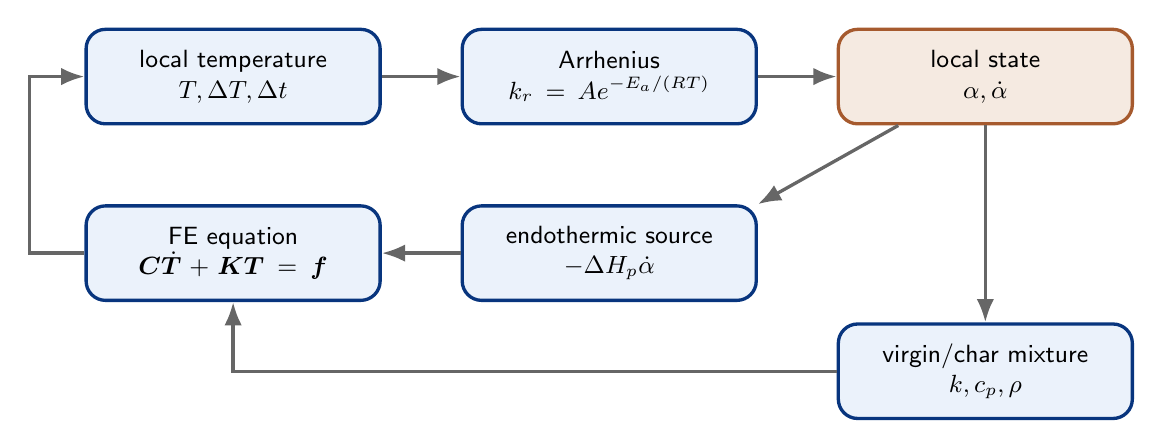
\begin{tikzpicture}[font=\sffamily\small,>=Latex,node distance=9mm and 10mm,
  block/.style={draw=B,very thick,rounded corners=7pt,fill=b!10,
    align=center,text width=35mm,minimum height=12mm},
  state/.style={draw=phenolicA,very thick,rounded corners=7pt,fill=phenolicB!18,
    align=center,text width=35mm,minimum height=12mm},
  arr/.style={-Latex,very thick,draw=black!60}]
  \node[block] (temp) {local temperature\\\(T,\Delta T,\Delta t\)};
  \node[block,right=of temp] (arrh) {Arrhenius\\\(k_r=Ae^{-E_a/(RT)}\)};
  \node[state,right=of arrh] (alpha) {local state\\\(\alpha,\dot\alpha\)};
  \node[block,below=25mm of alpha] (mix) {virgin/char mixture\\\(k,c_p,\rho\)};
  \node[block,below left=10mm and 10mm of alpha] (source) {endothermic source\\\(-\Delta H_p\dot\alpha\)};
  \node[block,left=of source] (fem) {FE equation\\\(\vect C\dot{\vect T}+\vect K\vect T=\vect f\)};
  \draw[arr] (temp)--(arrh); \draw[arr] (arrh)--(alpha);
  \draw[arr] (alpha)--(mix); \draw[arr] (alpha)--(source.north east);
  \draw[arr] (mix)-|(fem); \draw[arr] (source)--(fem);
  \draw[arr] (fem.west) -- ++(-7mm,0) |- (temp.west);
\end{tikzpicture}
\caption{Local coupling in Simulation 1. Conversion modifies both the heat
source and the properties at the following substep.}
\label{fig:sim1-coupling}
\end{figure}

\subsection{Simulation 1 Results (to be completed)}

\placeholder{Subsection reserved for results: temperatures, SVAR1, SVAR2,
pyrolysis depth, energy balances, and mesh-independence study.}

% ============================================================================
\clearpage
\section{Simulation 2: Outgassing and Element Deactivation in Mechanical}

\subsection{Proposed Theory and Derivation}

\subsubsection{Solid Mass Balance and Gas Generation}

Simulation 2 retains the kinetics used in Simulation 1, but distinguishes the
solid residue from the gaseous products. Over an initial volume, the loss of
condensed-phase mass is the gas source:
\begin{equation}
  \frac{\pd\rho_s}{\pd t}=-\dot\omega'''_g,
  \qquad
  \dot\omega'''_g=(\rho_v-\rho_c)\dot\alpha.
  \label{eq:solid-mass-sim2}
\end{equation}
The final gas yield of the single-reaction model is therefore
\begin{equation}
  Y_g=\frac{\rho_v-\rho_c}{\rho_v}=1-\frac{\rho_c}{\rho_v}.
  \label{eq:gas-yield}
\end{equation}
With the current tables, \(Y_g\) ranges from 0.44 to 0.48. A nominal value of
\(Y_g=0.47\) is consistent with the model, but must be confirmed using the
residual mass measured by TGA.

In a complete porous-ablator model, conservation of gas mass is written as
\begin{equation}
  \frac{\pd(\phi\rho_g)}{\pd t}
  +\vect\nabla\cdot(\rho_g\vect u_g)=\dot\omega'''_g,
  \label{eq:gas-mass-full}
\end{equation}
where \(\phi\) is the porosity and \(\vect u_g\) is the superficial velocity.
For slow flow through the char, Darcy's law and the ideal-gas law give
\begin{equation}
  \vect u_g=-\frac{K(\alpha,T)}{\mu_g}\vect\nabla p_g,
  \qquad
  \rho_g=\frac{p_g M_g}{R T_g}.
  \label{eq:darcy-ideal}
\end{equation}
Ablative-material response codes such as CHAR solve coupled forms of these mass
and energy balances~\cite{amar2010,amar2016,ewing2013}. A standard thermal
element in Mechanical, however, has no pressure degree of freedom. Consequently,
\code{UserMatTh} cannot solve Equation~\eqref{eq:gas-mass-full} by itself.
Remaining within Mechanical therefore requires either a substantially more
complex user-defined multiphysics element or a reduced-order model.

\subsubsection{Reduced Radial Closure Compatible with Mechanical}

The proposed model assumes that the gases generated in \code{phe0} escape
rapidly toward the hot wall and that their accumulation is negligible. In
cylindrical axisymmetry, the gas mass flux reaching the surface at radius
\(r_s\) is then obtained directly by integrating the source:
\begin{equation}
  \boxed{\dot m''_g(r_s)=\frac{1}{r_s}
  \int_{r_s}^{R_0}\dot\omega'''_g(r)\,r\,\dd r,}
  \label{eq:radial-gas-flux}
\end{equation}
where \(R_0\) is the outer boundary of \code{phe0}. This expression follows
from the balance \(2\pi r_sL\dot m''_g=\int_{r_s}^{R_0}2\pi rL
\dot\omega'''_g\dd r\). It conserves total gas mass even when pressure is not
solved explicitly.

The gas carries sensible enthalpy. A minimal local closure adds the following
term to the solid energy equation:
\begin{equation}
  \dot q_{m,g}=-\frac{\dot\omega'''_g}{\rho_s}
  c_{p,g}(T-T_\mathrm{ref}).
  \label{eq:gas-local-sink}
\end{equation}
This term must be used only if \(\Delta H_p\) does not already include this
enthalpy; otherwise it would be counted twice. A more faithful formulation adds
\(-\vect\nabla\cdot(\dot m''_g h_g)\) to the energy balance, as is done in
material-response models~\cite{ewing2013,amar2010}.

\subsubsection{Reduction of Convective Heat Flux by Blowing}

Outgassing into the chamber produces a blowing flow that opposes heat transfer.
For a steady, planar gas film with constant properties, the source-free energy
equation is
\begin{equation}
  \dot m''_g c_{p,g}\frac{\dd T}{\dd y}
  =k_g\frac{\dd^2T}{\dd y^2}.
\end{equation}
Integrating between the wall and the outer edge of the film, and expressing the
film thickness in terms of the no-blowing coefficient \(h_0=k_g/\delta\), gives
the classical correction in the form
\begin{equation}
  B_h=\frac{\dot m''_g c_{p,g}}{h_0},\qquad
  F(B_h)=\frac{B_h}{\exp(B_h)-1},
\end{equation}
\begin{equation}
  \boxed{q''_\mathrm{conv}=h_0F(B_h)(T_g-T_s).}
  \label{eq:blowing}
\end{equation}
Because \(F(0)=1\) and \(F(B_h)<1\) for \(B_h>0\), the model recovers the
current convection condition in the absence of outgassing and progressively
reduces the heat flux as gas production increases. This law is an engineering
closure; it does not replace a boundary-layer calculation and must be calibrated
against chamber pressure, propellant composition, and test data.

\subsubsection{Surface Balance, Recession, and Element-Deactivation Criterion}

Pyrolysis produces char; it does not automatically remove that char. Recession
requires a second mechanism---oxidation, sublimation, or mechanical erosion---
and a surface energy balance:
\begin{equation}
  q''_\mathrm{conv}+q''_\mathrm{rad}
  =q''_\mathrm{cond}+\dot m''_g\Delta h_g
   +\dot m''_\mathrm{abl}H_\mathrm{eff}.
  \label{eq:surface-balance}
\end{equation}
In the absence of sufficient chemical data, the following bounded,
energy-controlled law is proposed:
\begin{equation}
  \dot m''_\mathrm{abl}=
  \max\left[0,
  \frac{q''_\mathrm{conv}+q''_\mathrm{rad}-q''_\mathrm{cond}
  -\dot m''_g\Delta h_g}{H_\mathrm{eff}}\right],
  \qquad
  \dot s=\frac{\dot m''_\mathrm{abl}}{\rho_c}.
  \label{eq:recession}
\end{equation}
The recession depth is \(s(t)=\int_0^t\dot s\dd t\). The \code{phe0} elements
are arranged in radial bands; a band is deactivated only when \(s\) exceeds its
cumulative thickness. The criterion is therefore the integrated recession,
possibly combined with \(\alpha\ge0.99\), but never \(\alpha=1\) alone.

In MAPDL, \code{EKILL} multiplies an element's contribution by a near-zero
factor; the element remains in the mesh. A deactivated thermal element no longer
contributes heat capacity or applied loads, and its state variables are reset
when it is killed~\cite{ansys-birthdeath,ansys-ekill}. Any residual mass and
energy must therefore be recorded before \code{EKILL} and included in the
balance. After each band is deactivated, the hot-side convection and surface
elements must be transferred to the newly exposed face. With only eight layers
through \code{phe0}, recession would advance in increments of approximately
\SI{0.318}{mm}. A credible recession study should use 20 to 40 radial bands, or
demonstrate that the existing increment is sufficiently small.

\begin{figure}[H]
\centering
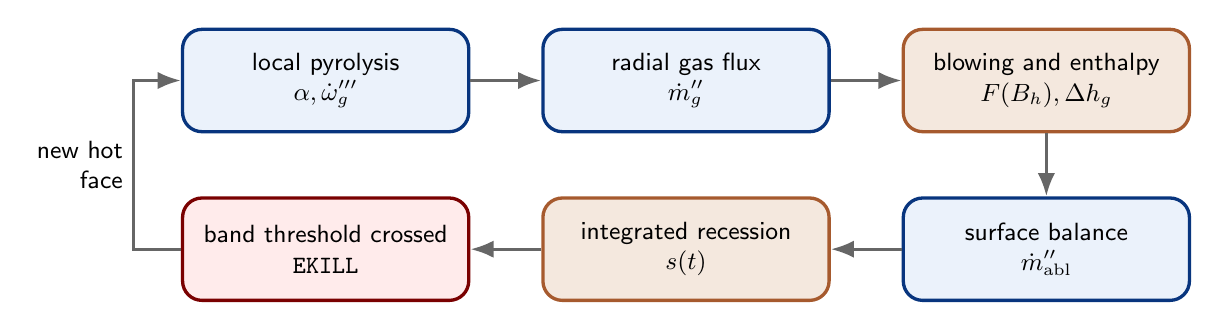
\begin{tikzpicture}[font=\sffamily\small,>=Latex,node distance=8mm and 9mm,
  block/.style={draw=B,very thick,rounded corners=7pt,fill=b!10,
    align=center,text width=34mm,minimum height=13mm},
  special/.style={draw=phenolicA,very thick,rounded corners=7pt,fill=phenolicB!20,
    align=center,text width=34mm,minimum height=13mm},
  kill/.style={draw=r,very thick,rounded corners=7pt,fill=red!8,
    align=center,text width=34mm,minimum height=13mm},
  arr/.style={-Latex,very thick,draw=black!60}]
  \node[block] (pyro) {local pyrolysis\\\(\alpha,\dot\omega'''_g\)};
  \node[block,right=of pyro] (gas) {radial gas flux\\\(\dot m''_g\)};
  \node[special,right=of gas] (blow) {blowing and enthalpy\\\(F(B_h),\Delta h_g\)};
  \node[block,below=of blow] (surface) {surface balance\\\(\dot m''_\mathrm{abl}\)};
  \node[special,left=of surface] (recession) {integrated recession\\\(s(t)\)};
  \node[kill,left=of recession] (ekill) {band threshold crossed\\\code{EKILL}};
  \draw[arr] (pyro)--(gas); \draw[arr] (gas)--(blow);
  \draw[arr] (blow)--(surface); \draw[arr] (surface)--(recession);
  \draw[arr] (recession)--(ekill);
  \draw[arr] (ekill.west) -- ++(-6mm,0) |- (pyro.west)
    node[pos=.25,left,align=right] {new hot\\face};
\end{tikzpicture}
\caption{Proposed physical sequence for Simulation 2 in Mechanical. Element
deactivation is driven by recession, not directly by SVAR1.}
\label{fig:sim2-chain}
\end{figure}

\subsubsection{Proposed Initial Values and Sensitivity Studies}

Table~\ref{tab:sim2-values} provides an initial parameter set for prototyping,
not for qualification. The permeability values are taken from the CHAR PICA
model and are only surrogates for a dense phenolic~\cite{amar2016}. Phenolic
resin products include, among others, \(\mathrm{H_2}\), water vapor, and aromatic
hydrocarbons, and depend on heating rate~\cite{bessire2023}; representing them
with a single pseudo-species is therefore a major simplification.

\begin{table}[H]
\centering
\scriptsize
\renewcommand{\arraystretch}{1.18}
\begin{tabular}{L{0.18\textwidth}M{0.16\textwidth}M{0.18\textwidth}L{0.38\textwidth}}
\toprule
\textbf{Quantity} & \textbf{Proposed nominal} & \textbf{Sensitivity range} & \textbf{Rationale / required measurement} \\
\midrule
Gas yield \(Y_g\) & 0.47 & 0.44--0.50 & Derived from the current virgin/char densities using Equation~\eqref{eq:gas-yield}; replace with TGA data. \\
Virgin porosity \(\phi_v\) & 0.13 & 0.05--0.20 & Derived from \(1-\rho_v/\rho_\mathrm{skeletal}\), with \(\rho_\mathrm{skeletal}=\SI{1430}{kg.m^{-3}}\), a historical phenolic--nylon value~\cite{clark1972}. \\
Char porosity \(\phi_c\) & 0.55 & 0.45--0.65 & Same calculation using \(\rho_c=\SIrange{600}{700}{kg.m^{-3}}\); measure by pycnometry/porosimetry. \\
Virgin permeability \(K_v\) & \(10^{-12}\ \mathrm{m^2}\) & \(10^{-14}\)--\(10^{-11}\ \mathrm{m^2}\) & PICA ``Model A'' value used as a surrogate~\cite{amar2016}; not transferable without testing. \\
Char permeability \(K_c\) & \(10^{-10}\ \mathrm{m^2}\) & \(10^{-12}\)--\(10^{-9}\ \mathrm{m^2}\) & Same source; logarithmic interpolation with respect to \(\alpha\) is recommended. \\
Gas viscosity \(\mu_g\) & \(4\times10^{-5}\ \mathrm{Pa\,s}\) & \(2\)--\(6\times10^{-5}\ \mathrm{Pa\,s}\) & Provisional hot pseudo-gas value; a mixture calculation is required. \\
Molar mass \(M_g\) & \(\SI{0.024}{kg.mol^{-1}}\) & 0.018--0.030 & Pseudo-species spanning light gases and vapor; calculate from the measured composition. \\
Gas heat capacity \(c_{p,g}\) & \(\SI{1.5}{kJ.kg^{-1}.K^{-1}}\) & 1.2--2.0 & Initial pseudo-gas value; use a \(c_p(T,p)\) table after characterization. \\
Char emissivity \(\varepsilon_c\) & 0.80 & 0.70--0.90 & Historical phenolic--nylon starting point~\cite{clark1972}; high-temperature measurement required. \\
Ablation enthalpy \(H_\mathrm{eff}\) & \(\SI{35}{MJ.kg^{-1}}\) & 20, 35, and \(\SI{50}{MJ.kg^{-1}}\) & Effective recession parameter. \SI{50}{MJ.kg^{-1}} is a historical sublimation anchor~\cite{clark1972}; calibrate against thickness loss. \\
Reference temperature \(T_\mathrm{ref}\) & \(\SI{295.15}{K}\) & fixed & Consistent with the initial state. \\
Recession increment & \(\dot s\Delta t\le0.2\Delta r\) & 0.1--0.25 \(\Delta r\) & Numerical criterion to prevent several bands from being crossed in one substep. \\
\bottomrule
\end{tabular}~\\[1em]
\caption{Proposed initial parameters for Simulation 2. They must be treated as
uncertain variables until they have been characterized.}
\label{tab:sim2-values}
\end{table}

Before a complete motor simulation is attempted, three separate validation
campaigns are required: (i) \mbox{TGA/DSC/LFA} coupon testing for decomposition,
(ii) permeability and gas-pressure measurements in a heated coupon for
outgassing, and (iii) an instrumented flame or motor test for \(h_0\), blowing,
and recession. The model must not compensate for an incorrect chamber boundary
condition by artificially adjusting \(H_\mathrm{eff}\).

\subsection{Implementation in Mechanical (to be completed)}

\placeholder{Subsection reserved for the future implementation: band
architecture, MAPDL commands, load transfer, restart logic, and conservation
checks.}

\subsection{Simulation 2 Results (to be completed)}

\placeholder{Subsection reserved for the results: outgassing mass flow rate,
blowing factor, recession, chronology of deactivated bands, and mass and energy
balances.}

% ============================================================================
\clearpage
\renewcommand{\refname}{References}
\renewcommand{\bibname}{References}
\begin{thebibliography}{99}

\bibitem{ansys-usermatth}
ANSYS, Inc., \emph{UserMatTh --- User-Defined Thermal Material Model},
Mechanical APDL Programmer's Reference, version 2026 R1,
\url{https://ansyshelp.ansys.com/public/Views/Secured/corp/v261/en/ans_prog/Z7K4r1e5lcd.html},
accessed July 15, 2026.

\bibitem{ansys-birthdeath}
ANSYS, Inc., \emph{Using Element Birth and Death}, Mechanical APDL Advanced
Analysis Guide,
\url{https://ansyshelp.ansys.com/public/Views/Secured/corp/v251/en/ans_adv/Hlp_G_ADV6_2.html},
accessed July 15, 2026.

\bibitem{ansys-ekill}
ANSYS, Inc., \emph{EKILL --- Deactivates an element}, Mechanical APDL Command
Reference,
\url{https://ansyshelp.ansys.com/public/Views/Secured/corp/v242/en/ans_cmd/Hlp_C_EKILL.html},
accessed July 15, 2026.

\bibitem{ewing2013}
M. E. Ewing, T. S. Laker, and D. T. Walker, \emph{Numerical Modeling of
Ablation Heat Transfer}, NASA NTRS 20140008557, 2013,
\url{https://ntrs.nasa.gov/citations/20140008557}.

\bibitem{amar2010}
A. J. Amar, N. D. Calvert, and B. S. Kirk, \emph{Development and Verification of
the Charring Ablating Thermal Protection Implicit System Solver}, NASA NTRS
20110000471, 2010,
\url{https://ntrs.nasa.gov/citations/20110000471}.

\bibitem{amar2016}
A. J. Amar, A. B. Oliver, B. S. Kirk, G. Salazar, and J. Droba,
\emph{Overview of the CHarring Ablator Response (CHAR) Code}, NASA NTRS
20160005889, 2016,
\url{https://ntrs.nasa.gov/citations/20160005889}.

\bibitem{clark1972}
R. K. Clark, \emph{A Numerical Analysis of the Transient Response of an
Ablation System Including Effects of Thermal Nonequilibrium, Mass Transfer and
Chemical Kinetics}, NASA-TM-X-68853, NASA NTRS 19730002381, 1972,
\url{https://ntrs.nasa.gov/citations/19730002381}.

\bibitem{bessire2023}
B. K. Bessire, \emph{Analysis of Pyrolysis Products from Ablative TPS}, NASA
NTRS 20230000843, 2023,
\url{https://ntrs.nasa.gov/citations/20230000843}.

\bibitem{nasa-testing}
NASA Ames Research Center, \emph{Thermal Protection Materials Branch ---
Testing and Fabrication}, description of TGA, DSC, and LFA measurements,
\url{https://www.nasa.gov/thermal-protection-materials-branch-testing-and-fabrication/},
accessed July 15, 2026.

\bibitem{local-step}
MIT Rocket Team, \code{motoren.stp}, project AP214 STEP geometry, local file
analyzed July 15, 2026.

\bibitem{local-model}
MIT Rocket Team, \code{EngineeringData.xml}, \code{ds.dat},
\code{phenolic_pyrolysis_native.apdl}, and \code{usermatth.F}, local artifacts
from the ANSYS Mechanical 2026 R1 simulation, state analyzed July 15, 2026.

\end{thebibliography}

\clearpage
\renewcommand{\listfigurename}{List of Figures}
\renewcommand{\listtablename}{List of Tables}
\listoffigures
\listoftables

\vfill
\section*{AI Usage Statement}

Artificial intelligence was used to generate portions of this document and to
assist with part of its technical content development.
\end{document}
